
%%This is a very basic article template.

%%There is just one section and two subsections.

\documentclass[12pt]{article}

\usepackage[slovak]{babel}
\usepackage[utf8]{inputenc}
\usepackage{amsmath}
%%\usepackage[dvipdfm]{graphicx}
\usepackage{graphicx}
\usepackage{bmpsize}
\usepackage{pdfpages}
\usepackage{wrapfig}
\usepackage{setspace}
\usepackage{esvect}
\usepackage[top=2.54cm, bottom=2.54cm, left=3.5cm, right=2.0cm]{geometry}

\setstretch{1.5}

\begin{document}

\title{Rozpoznávanie dopravných značiek}

\author{Mário Kapusta}
%% titulka s informaciami
\maketitle
\thispagestyle{empty}
\clearpage
%% obsah
\tableofcontents
\addtocontents{toc}{\protect\thispagestyle{empty}}
\thispagestyle{empty}
\clearpage
%%zoznam tauliek
\listoftables
\thispagestyle{empty}
\clearpage
%%zoznam orazkov
\listoffigures
\thispagestyle{empty}
\clearpage
%% astrakt
\begin{abstract}
V praci sme sa zaoberali\ldots
\end{abstract}
\clearpage

%% zaciatok prace
%%\section{Počítačové videnie}
%%\subsection{História počítačového videnia}
%%\subsection{Hlavné témy počítačového videnia}
%%\subsubsection{Transformácia}
%%\subsubsection{Filtrovanie a kompresia}
%%\subsubsection{Vylepšovanie obrazu}
%%\subsubsection{Rozpoznávanie objektov}
%%\subsubsection{Pozíciovanie}
%%\subsection{Technológie}
%%\subsubsection{OpenCV}
%% http://simplecv.tumblr.com/post/19307835766/opencv-vs-matlab-vs-simplecv
%%\subsubsection{Matlab}
%%\subsubsection{SimpleCV}

\section{Rozpoznávanie objektov}
\paragraph{}
Rozpoznávanie objektov v počítačovom videní sa zaoberá problematikou rozpoznania už bežne známych objektov v reálnom svete, pomocou technológií.
Táto úloha je prekvapivo ťažká. Ľudia vedia rozpoznávať objekty reálneho sveta bez námahy a okamžite. Problém nastáva však pri algoritmickom opise tejto úlohy, ktorej by chápali stroje.
\cite{machine_vission}
\paragraph{}
Okrem zložitého algoritmického problému, tu existuje aj skutočnosť, že pre kvalitné rozpoznanie akéhokoľvek objektu sme taktiež závislí na hardware.
Keďže rozpoznávame z obrazu, tento obraz je potrebné zachytávať kamerou. Čím lepšie vie kamera pracovať so svetlom a má kvalitnejšie parametre, tým je väčšia šanca že rozpoznanie objektu bude kvalitnejšie.
Pri rozpoznávaní objektov je veľmi dôležité aj umiestnenie kamery. Tam platí, čím kolmejšie k objektu je kamera smerovaná, tým je objekt viac viditeľný a tak aj ľahšie rozpoznateľný. 
\cite{machine_vission}
\paragraph{}
Problematika rozpoznávania objektov sa ďaľej delí na konkrétnejšie problémy. V našom prípade sa jedná o problematiku rozpoznávania dopravných značení.
\cite{machine_vission}
%%http://www.cse.usf.edu/~r1k/MachineVisionBook/MachineVision.files/MachineVision_Chapter15.pdf
\subsection{Rozpoznávanie dopravných značení}
\paragraph{}
Problematika rozpoznávania dopravných značení je pomerne nová a pri písaní práce som tak mohol čerpať len z veľmi malého počtu literatúry, zaoberajúcou sa touto témou.
Bol som donútený študovať prolematiku podrobne a vytvoriť riešenie, hlavne na poznatkoch z rozpoznávania iných objektov.
Popri tvorbe práce, vznikali rôzne ďaľšie práce a publikácie zaoberajúce sa konkrétne témou rozpoznávania dopravných značení.
Nebolo však možné sledovať všetky nové objavy a zistenia v tejto oblasti, ktoré vznikali popri tvorbe tejto bakalárksej práci.
Rozbor témy rozpoznávania dopravných značení je tak postavený hlavne na informáciách z jesene 2012.
\paragraph{}
Výskum témy rozpoznávania dopravných značení má v praxi silné uplatnenie. V oblasti dopravy, by to znamenalo pomoc vodičom vnímať a rozpoznávať, dopravné značenia, ktoré si vodič nevšimol, nepochopil poprípade im nerozumie.
Napriek tomu, že máme k dispozícii už dlhý výskum v oblasti počítačového videnia a množstvo kvalitného hardwaru, je úloha rozpoznávania dopravných značení pomerne zložitá.
Skutočnosť, že systém musí reagovať pomerne rýchlo na dynamické zmeny ktoré pri jazde autom nastávajú a taktiež s rôznorodým pozadím a viditeľnosťou, ktoré nám prostredie vytvára,
nám vytvára komplexnú problematiku v počítačovom videní, ktorej sa oplatí venovať pozornosť.\cite{tfs_pdf}
\paragraph{}
Konkrétne, problematika rozpoznávania dopravných značiek obsahuje dve fázy, z ktorých sa celý proces skladá:
\begin{enumerate}
  \item \textbf{Detekcia dopravného značenia} - detekuje umiestnenie dopravného značenia v obraze.
  \item \textbf{Rozpoznanie detekovaného dopravného značenia} - rozpoznáva významovú hodnotu dopravného značenia.
\end{enumerate} 
Existuje viac techník pre detekciu dopravných značení, ale ako najúčinnejšia metóda sa ukázalá farebná segmentácia a následné rozpoznanie podľa tvaru.
Pri získavaní významovej hodnoty značky je najefektívnejšie využiť neurónové siete.
\cite{tfs_pdf}
\paragraph{}
Prvý rozpoznávač dopravných značení bol do praxe nasadený v roku 2008, spoločnosťou BMW.\cite{bmw} Nasledujúci rok nasadila svoj prvý systém pre rozpoznávanie dopravných značení aj spoločnosť Mercedes.\cite{mercedes}
Tieto prvé rozpoznávače dopravných značení vedeli rozpoznávať len značky ktoré hovorili o rýchlostnom obmedzení. Hneď na to boli tieto automobilky nasledované ďalšími konkurentami, ktorí systém rozpoznávania vylepšovali o rôzne funkcionality.
Od roku 2012 vyvýja firma Volvo komplexný systém rozpoznávania dopravných značení pomocou počítačového videnia, ktorý nazvala Road Sign Information. Tento systém je implementovaný vo všetkých nových modeloch spomínanej automobilky.\cite{volvo}
%%nieco odbornejsie este
\subsection{Rozpoznávanie iných objektov}
Rozpoznávanie jednotlivých objektov v obraze spočíva v tom, objaviť potrebné obrazové regióny hľadaného modelu, pričom sa snažiť ignorovať pozadie.
Tieto regióny sú však pre každý objekt iné. Niekedy je potrebné sledovať farbu, inokedy tvary alebo pohyb. Pri niektorých špecifických objektoch je potrebné hľadať rôzne body a počítať uhly, ktoré zvierajú.
Medzi tieto špecifickejšie objekty patrí napríklad problematika rozpoznávania tvárí.
\cite{object_rec_scene}
\subsubsection{Rozpoznávanie tvárí}
Proces rozpoznávania tvárí je postavený na takom princípe, že sa snažíme hľadať už známe kontrasty medzi regiónmy na tváry a ich priestorových vzťahov ktoré vyjadrujú.
Tieto vzťahy nie sú také jednoznačné a tak sa museli vypracovať algoritmy, a spôsoby ktoré problematiku riešia. 
Najpoužívanejšia metóda je používať neurónovú sieť, ktorej posielame vzorky správnych a nesprávnych vzťahov a naučíme stroj rozpoznávať tváre sám.
V súčasnosti už nie je problém nájsť takúto technológiu použítú kdekoľvek vo svete.
\cite{object_detection_viola}
\section{Výskum}
\paragraph{}
Cieľom práce je vypracovať komplexný návrh riešenia pre vyhľadávanie a rozpoznávanie dopravného značenia a taktiež vytvoriť funkčnú aplikáciu, ktorá
bude schopná rozpoznať zvislé dopravné značenia. Táto aplikácia bude naprogramovaná v jazyku Java a bude spustiteľná na
 operačnom systéme Android 2.3, ktorý je určený pre mobilné zariadenia. Computer vision (počítačové videnie), nám zaručí open-source knižnica OpenCV.
\subsection{Matematické metódy}
\paragraph{}
Mnoho matematických metód sa bude priamo vysvetlovať pri predstavovaní danej OpenCV funkcionality.
V tejto sekcii si predstavíme také matematické metódy ktoré nám pomůžu lepšie sa orientovať pri opise konkrétnych funkcionalít OpenCV.
\subsubsection{Konvolúcia}
\paragraph{}
Konvolúcia je matematická metóda, ktorá systematicky prechádza celý obraz a na výpočet novej hodnoty bodu využíva malé okolie \emph{O} reprezentatívneho bodu. 
Táto hodnota je zapísaná do nového obrazu. Diskrétna konvolúcia má tvar:
\begin{align*}
g(x,y) = \sum_{(m,n)} \sum_{(e^0)} h(x - m,y - n)f(m,n)
\end{align*}
kde f predstavuje obrazovú funkciu pôvodného obrazu, g predstavuje obrazovú funkciu nového obrazu, h predstavuje konvolučnú masku alebo konvolučné jadro, h nám udáva koeficienty jednotlivých bodov v okolí O.
Najčastejšie sa používajú  obdĺžníkové masky s nepárnym počtom riadkov a stĺpcov, pretože v tom prípade môže reprezentatívny bod ležať v strede masky.
\paragraph{}
Transformácie v lokálnom okolí bodu sa delia na dve skupiny: \\
\textbf{Vyhladzovanie} – tieto metódy sa snažia potlačiť šum v obraze, ale rozostrujú hrany. \\
\textbf{Ostrenie} – detekcia hrán a čiar, ale zosilňuje šum. \\
\paragraph{}
Podľa matematických vlastností môžeme metódy predspracovania rozdeliť na \\
\textbf{Lineárne metódy} – novú jasovú hodnotu bodu počítajú ako lineárnu kombináciu vstupných bodov. Napr.: priemerovací filter \\
\textbf{Nelineárne metódy} – berú do úvahy len body s určitými vlastnosťami. Napr.: mediánový filter.
\cite{DIP}
\subsubsection{Aproximácia}
\paragraph{}
Aproximácia je matematická metóda pri ktorej sa snažíme vyjadriť zložitú funkciu jednoducho. Túto metódu sa snažíme uskutočniť aritmetickými operáciami, ktoré dokze uskutočniť počítač.
Jednou z najlepšou metódou vyjadrenia funkcie jednoduchšie je cez polynómy, čo sú vlastne najjednoduchšie funkcie, ktoré možno na počítači vypočítať priamo. Taktiež sa dajú ľahko integrovať a derivovať a vo všeobecnosti sa s nimi jednoducho zaobchádza.
Každá aproximácia je presná na určitom intervale, mimo intervalu sú funkcie odlišné.
\cite{aproximacia}
\paragraph{}
Predstavme si, že našou úlohou je opísať rozloženie pôdneho znečistenia istou chemikáliou. K dispozícii máme samozrejme meracie prístroje. Jednotlivými vrtmi odoberáme vzorky pôdy, ktoré potom podrobíme analýze.
Prolém spočíva v tom, že nie je možné, aby sme takto zmapovali celú oblesť dokonale, keďze sme časovo aj finančne obmedzení. Takže našou úlohou bude dostať dostatočne presný opis znečistenia celého územia z konečného počtu meráni.
Musíme tak nejakým spôsobom preniesť namerané hodnoty na celú oblasť. O toto sa nám stará aproximácia. Existuje mnoho spôsobov ako tento prenos uskutočniť. Voľba metódy závisí od konkrétnej situácie.
\cite{num_metody}
\paragraph{}
Existuje niekoľko delení aproximácie, predstavíme si niekoľko základných typov a delení. Výber danej metódy závisí od konkrétneho problému.
\begin{enumerate}
  \item Rozdelenie aproximácií podľa aproximačnej funkcie
	\begin{itemize}
	  \item \textbf{Lineárny typ}
		\begin{align*}
		f(x) \approx a_0 g_0(x) + a_1 g_1(x) + \ldots + a_m g_m(x)
		\end{align*}
	  \item \textbf{Racionálny typ}
	  	\begin{align*}
		f(x) \approx \frac{a_0 g_0(x) + a_1 g_1(x) + \ldots + a_m g_m(x)}{b_0 g_0(x) + b_1 g_1(x) + \ldots + b_m g_m(x)}
		\end{align*}
	\end{itemize}
  \item Rozdelenie aproximácií podľa zvolených konštánt
  	\begin{itemize}
	  \item 
	  	\textbf{Interpolačná aproximácia} - Pri interpolácii si vyberieme nejaké body na vzore, čo je vlastne zložitá funkcia, z ktorej chceme dostať jednoduchšiu, napríklad obraz.
	  	Obraz musí tými bodmi na vzore prechádzať. Funkcie musia mať rovnakú deriváciu v danom bode.
	  \item 
	  	\textbf{Aproximácia metódou najmenších štvorcov} - Funkcia \emph{f(x)} a jej aproximácia majú pri tomto type aproximácie podobný obsah pod krivkou.
	  \item 
	  	\textbf{Čerbyševova aproximácia} - Tento typ aproximácie sa snaží o najmenší rozdiel medzi funkciou \emph{f(x)} a jej aproximáciou v určitom intervale.
	\end{itemize}
\end{enumerate}
V našej práci budeme využívať aproximáciu nepriamo. Väčšinou pôjde o aproximáciu pomocou bodov a teda interpoláciu.
\cite{aproximacia}
\subsubsection{Greenová veta}
\paragraph{}
Greenová veta bude použitá v práci opäť nepriamo. Bude ju používať OpenCV knižnica napríklad na výpočet veľkosti ľubovolnej kontúry. Greenová veta nám umožnuje previesť výpočet krivkového integrálu druhého druhu po jednoduchej uzavretej krivke na výpočet dvojného integrálu.
\cite{mat_an_2}	\\ \\
	  	\textbf{Formulácia} - \emph{Nech \begin{math}D \subset R^2 \end{math} je regulárna uzavrená oblasť, \begin{math}\partial \vv{D} \end{math} kladne orientovaná hranica oblasti D. Nech \begin{math} F = (F_1,F_2) \end{math} je vektorové  pole triedy \begin{math} c^1 \end{math} v D. Potom platí:}
	  	\begin{align*}
		\int_{\partial \vv{D}} F d\vv{s} = \int\int_{D} \text{rot} F d \mu \text{,}
		\end{align*}
		\emph{kde \begin{math} \mu \end{math} značí Jordanovú mieru. V zložkovom tvare.} 
		\begin{align*}
		\int_{\partial \vv{D}} F_1 d x + F_2 d y = \int\int_{D} \left ( \frac{\partial f_2}{\partial x} - \frac{\partial f_1}{\partial y} \right ) dxdy \text{. \cite{mat_an_2}}
		\end{align*}
\subsection{Funkcionalita OpenCV}
\paragraph{}
OpenCV je open source knižnica počítačového videnia. Knižnica je napísaná v programovacích jazykoch C a C++. Aktívne sa pracuje na
rozhraniach pre Python, Ruby, Matlab, Javu a iných programovacích jazykoch. V našej práci sme sa sústredili na verziu pre programovací jazyk Java,
ktorý sa používa pri tvore aplikácii pre Android OS.
\cite{learning_opencv}
\paragraph{}
OpenCV knižnica bola navrhnutá tak, aby funkcie použité v tejto knižnici, boli čo najefektívnejšie a čo najviac zamerané na real-time aplikácie.
Knižnica je napísaná v optimalizovanom jazyku C a tak môže jednoducho využiť aj silu viacjadrových procesorov.
Taktiež existujú knižnice, špeciálne určené pre procesory s architektúrou Intel. IPP (Integrated Performance Primitives) knižnice  sa skladajú z nízko levelových 
optimalizovaných postupov a rôznych algoritmických olastí, ktoré pracujú na procesoroch s architektúrou Intel oveľa efektívnejšie.
\cite{learning_opencv}
\paragraph{}
Jeden z hlavných cieľov OpenCV je sprístupniť jednoducho použiteľné prostredie ktoré pomôže developerom ľahko a rýchlo budovať aplikácie s použitím počítačového videnia
pre rôzne použitia v oblasti, medicíny, bezpečnosti, robotiky, dopravy, priemyselnej výroby a iných, pre ktoré ma OpenCV dokonca aj špecifické funkcionality.
\cite{learning_opencv}
\paragraph{}
Pre olasť rozpoznávania ojektov sú taktiež mnohé špecifické funkcionality.
Pri problematike rozpoznávania zvislích dopravných značení sme niektoré z nich použili a preto je potrebné si pre lepšie pochopenie problematiky tieto funkcie vysveliť podrobnejšie.
\subsubsection{cvtColor}
\paragraph{}
Funkcia \emph{cvtColor} prevedie obraz z jedného farebného spektra do iného. Je to jedna z najpoužívanejších funkcií, keďže na rozpoznávanie objektov je potrené si obraz pripraviť
cez mnohé farebné filtre. Vstupné parametre je možné pozorovať pri tabuľke \ref{cvtColorPar}.
\cite{cvtColor}
\cite{OpenCVDoc}
\begin{table}
	\centering
    \begin{tabular}{ | l | l | p{5cm} |}
    \hline
    Premenná & Dátový typ & Popis \\ \hline
    src & Mat & Vstup je 8-bitový, 16-bitový obraz alebo formát čísla s plávajúcou desatinou čiarkou. \\ \hline
    dst & Mat & Výstupný obraz s rovnakými parametrami ako na vstupe. \\ \hline
    code & int & Farebné spektrum ktoré do ktorého požadujeme obraz previesť. \\
    \hline
    \end{tabular}
  	\caption{Tabulka znázorňuje vstupy funkcie cvtColor}
  	\label{cvtColorPar}
\end{table}
\paragraph{}
Pri používaní funkcie \emph{cvtColor}, je potrebné si určiť o akú konverziu ide. OpenCV, už má k dispozícii predpripravené konštanty, ktoré konverziu lepšie vyjadrujú.
Matematický prepočet si OpenCV už spraví v jadre. Konverzií je v OpenCV naprogramovaných už mnoho, my si predstavíme matematický model konverzie,
ktorú v našom prípade rálne využijeme. Jedná sa o konverziu z BGR(pri OpenCV je poradie kanálov pre model RGB zoradený opačne) do farebného modelu HSV a späť.
\cite{cvtColor}
\cite{OpenCVDoc}
\paragraph{} 
V prípade 8 a 16 bitového obrazu je potrené jednotlivé kanály R,G a B previesť do formátu s plávajúcou desatinou čiarkou a zmenšiť rozsah od 0 do 1.
\begin{table}
\begin{align*}
BGR \leftrightarrow HSV
\end{align*}
\begin{align*}
V \leftarrow max(R,G,B)
\end{align*}
\begin{align*}
S \leftarrow \begin{cases} \frac{V - min(R,G,B)}{V}, & \text{ pokiaľ } V \neq 0 \\ 0, & \text{ pokiaľ } V = 0 \end{cases} \\
\end{align*}
\begin{align*}
H \leftarrow \begin{cases} \frac{60(G - B)}{V - min(R,G,B)}, & \text{ pokiaľ } V = R \\ \frac{120 + 60(B - R)}{V - min(R,G,B)}, & \text{ pokiaľ } V = G \\ \frac{240 + 60(R - G)}{V - min(R,G,B)}, & \text{ pokiaľ } V = B \end{cases} 
\end{align*}
\begin{align*}
\text{ Pokiaľ } H < 0, & \text{ tak } H = H + 360
\end{align*}
\begin{align*}
\text{ Na výstup pôjde } 0 \le V \le 1, 0 \le S \le 1, 0 \le H \le 1
\end{align*}
\caption{Konverzia RGB modelu na HSV\cite{hsv_wiki_cz}\cite{cvtColor}\cite{OpenCVDoc}}
\label{cvtColorEquals}
\end{table}
\subsubsection{Canny}
\paragraph{}
Hlavná úloha funkcie \emph{Canny} je vyhľadávať okraje, kontúry a hrany všetkých objektov. Pri kombinácii s rôznymi filtrami, môžeme docieliť, vyhľadanie hrán úmyselného objektu.
Na rozoznávanie sa využíva algoritmus \emph{Canny86}.
\cite{canny}
\cite{OpenCVDoc}
\paragraph{}
Kontúrový alebo hranový detektor by mal spĺňať tri kritéria, ktoré určil John Canny.
\begin{enumerate}
  \item Detekčné kritérium, detektor nesmie zabudnúť na významnú hranu a na jednu hranu môže byť maximálne jedna odozva.
  \item Lokalizačné kritérium, rozdiel medzi skutočnou a nájdenou hranou má byť minimálny.
  \item Kritérium jednej odozvy.
\end{enumerate}
Cannyho detektor využíva konvolúciu s dvojrozmerným Gaussianom a deriváciu v smere gradientu.
Poskytuje informácie o smere a veľkosti hrany. Nech G je dvojrozmerný Gaussian. Nech Gn je prvá derivácia G v smere gradientu
\begin{align*}
G_n = \frac{\delta G}{\delta n} = n\bigtriangledown G
\end{align*}
kde n je smer gradientu, ktorý dostaneme nasledovne
\begin{align*}
n = \frac{\bigtriangledown(G * f)}{|\bigtriangledown(G * f)|}
\end{align*}
Hranu dostaneme v bode, kde funkcia \begin{math}\ G_n *f  \end{math} dosiahne lokálne maximum, a druhá derivácia sa rovná nule.
\begin{align*}
\frac{\delta^2}{\delta n^2} G * f = 0
\end{align*}
Pre silu hrany platí:
\begin{align*}
|G_n * f| = |\bigtriangledown (G * f)|
\end{align*}
Kritérium jednej odozvy sa dosahuje následne prahovaním. 
\cite{DIP}
\cite{JCanny}
\cite{canny_wiki_en}
\paragraph{}
Vstupné parametre je možné pozorovať pri tabuľke \ref{cannyPar}.
Najmenšia hodnota medzi \emph{threshold1} a \emph{threshold2} je použitá na prepájanie kontúr. Tá najväčšia hodnota je použitá ako začínajúci segment najsilnejších kontúr.
Pri správnom nastavení, sa dá dosiahnuť pomerne kvalitné odstránenie nepotrených kontúr.
\cite{canny}
\cite{OpenCVDoc}
\begin{table}
	\centering
    \begin{tabular}{ | l | l | p{5cm} |}
    \hline
    Premenná & Dátový typ & Popis \\ \hline
    image & Mat & Vstup je 8-bitový obraz s jedným farebným kanálom. \\ \hline
    edges & Mat & Výstup je mapa všetkých nájdených kontúr. \\ \hline
    threshold1 & double & Prvá prahová hodnota (threshold). \\ \hline
    threshold2 & double & Druhá prahová hodnota (threshold). \\
    \hline
    \end{tabular}
  	\caption{Tabulka znázorňuje vstupy funkcie canny}
  	\label{cannyPar}
\end{table}
%%\subsubsection{HoughLinesP}
%%nebolo v praci pouzite
\subsubsection{GaussianBlur}
\paragraph{}
Vyhladzuje obraz pomocou \emph{GaussianBlur} filtra.
\cite{gaussianblur_doc}
\cite{OpenCVDoc}
\paragraph{}
\emph{GaussianBlur} filter funguje na princípe \emph{N * N} konvolúcie pri ktorej sa každý pixel prehodnotí na základe \emph{Gaussian} funkcie.
Táto funkcia tak prevedie rozostrenie pre každý pixel obrazu.
\cite{gaussianblur}
\begin{align*}
H(x,y) = \frac{1}{2\pi\sigma^2}e^{\frac{(x^2)+(y^2)}{2\sigma^2}}
\end{align*}
\paragraph{}
Princíp konvolúcie 2D obrazu je postavený na tom, že sa systematicky snažíme spracovávať okolie pixelu a dostať výslednú hodnotu z okolia reprezentatívneho bodu.
Konvolúcia sa často používa pri spracovávaní obrazu, ako je vyhladzovanie obrazu, ostrenie, detekcia hrán a obrázkov.
\cite{convolution}
\cite{DIP}
\paragraph{}
Vstupné parametre pre \emph{GaussianBlur} je možné pozorovať pri tabuľke \ref{gaussianblurPar}. 
Pri premennej \emph{ksize} si môžeme napríklad nastaviť veľkosť matice, ktorá sa bude pri konvolúcii používať.
Veľkosť matice pri konvolúcii ovplivní rozostrenie. Čím väčšiu maticu používame, tím väčšie rozostrenie dostaneme.
\cite{gaussianblur_doc}
\cite{OpenCVDoc}
\begin{table}
	\centering
    \begin{tabular}{ | l | l | p{5cm} |}
    \hline
    Premenná & Dátový typ & Popis \\ \hline
    src & Mat & Vstup je obraz s ľubovolným počtom farebných kanálov. \\ \hline
    dst & Mat & Výstup s rovnakými parametrami ako bol vstup. \\ \hline
    ksize & Size & Veľkosť Gaussian jadra. Matica konvolúcie. \\ \hline
    sigmaX & double & Smerodajná odchýlka Gaussian jadra v smere X. \\ \hline
    sigmaY & double & Smerodajná odchýlka Gaussian jadra v smere Y. \\
    \hline
    \end{tabular}
  	\caption{Tabulka znázorňuje vstupy funkcie GaussianBlur}
  	\label{gaussianblurPar}
\end{table}
\subsubsection{inRange}
\paragraph{}
Funkcia \emph{inRange} zisťuje, či sa prvky poľa nachádzajú medzi prvkami ďalších dvoch polí.
\paragraph{}
Funkcia kontroluje rozsah nasledujúco:
\begin{itemize}
  \item Pre každý prvok vstupného pola s jedným kanálom
	\begin{align*}
	dst(I) = lowerb(I)_0 \le src(I)_0 \le upperb(I)_0
	\end{align*}
  \item Pre každý prvok vstupného pola s dvomi kanálmy
  	\begin{align*}
	dst(I) = lowerb(I)_0 \le src(I)_0 \le upperb(I)_0 \wedge lowerb(I)_1 \le src(I)_1 \le upperb(I)_1
	\end{align*}
  \item A tak ďaľej\ldots
\end{itemize}
\paragraph{}
Vstupné parametre pre \emph{inRange} je možné pozorovať pri tabuľke \ref{inRangePar}. 
\cite{inrange_doc}
\cite{OpenCVDoc}
\begin{table}
	\centering
    \begin{tabular}{ | l | l | p{5cm} |}
    \hline
    Premenná & Dátový typ & Popis \\ \hline
    src & Mat & Vstupné zdrjové pole. \\ \hline
    lowerb & Scalar & Spodná hranica poľa alebo skalárna veličina. \\ \hline
    upperb & Scalar & Vrchná hranica poľa alebo skalárna veličina. \\ \hline
    dst & Mat & Výsledné pole, rovnako veľké ako vstup. \\
    \hline
    \end{tabular}
  	\caption{Tabulka znázorňuje vstupy funkcie inRange}
  	\label{inRangePar}
\end{table}
\subsubsection{bitwise\_not}
\paragraph{}
Je jednoduchá funkcia, ktorá invertuje všetky bity v poli ktoré jej pošlete. Taktiež má aj jednoduché vstupné parametre, ktoré vidieť aj v tauľke \ref{bitwisePar}.
\cite{bitwise_not_doc}
\cite{OpenCVDoc}
\begin{table}
	\centering
    \begin{tabular}{ | l | l | p{5cm} |}
    \hline
    Premenná & Dátový typ & Popis \\ \hline
    src & Array & Vstupné pole plné bitov. \\ \hline
    dst & Array & Výstupné pole plné invetovaných bitov \\
    \hline
    \end{tabular}
  	\caption{Tabulka znázorňuje vstupy funkcie bitwise\_not}
  	\label{bitwisePar}
\end{table}
\subsubsection{threshold}
\paragraph{}
Aplikuje pevnú prahovú úrovní pre každý prvok poľa. Zvyčajne sa používa na získanie binárnej úrovne obrazu v odtieňoch sivej, alebo pre odstránenie šumu.
Funkcia \emph{treshold} funguje na princípe filtrovania pixelov ktoré majú príliž veľkú, alebo príliž malú hodnotu. Existuje niekoľko možností ako tento šum odstrániť.
\begin{itemize}
  \item THRESH\_BINARY
	\begin{align*}
	dst(x,y) = \begin{cases} maxval, & \text{ pokiaľ } src(x,y) > tresh \\ 0, & \text{ inak } \end{cases} \\
	\end{align*}
  \item THRESH\_BINARY\_INV
  	\begin{align*}
	dst(x,y) = \begin{cases} 0, & \text{ pokiaľ } src(x,y) > tresh \\ maxval, & \text{ inak } \end{cases} \\
	\end{align*}
  \item THRESH\_TRUNC
  	\begin{align*}
	dst(x,y) = \begin{cases} trashold, & \text{ pokiaľ } src(x,y) > tresh \\ src(x,y), & \text{ inak } \end{cases} \\
	\end{align*}
  \item THRESH\_TOZERO
  	\begin{align*}
	dst(x,y) = \begin{cases}  src(x,y), & \text{ pokiaľ } src(x,y) > tresh \\ 0, & \text{ inak } \end{cases} \\
	\end{align*}
  \item THRESH\_TOZERO\_INV
  	\begin{align*}
	dst(x,y) = \begin{cases} 0, & \text{ pokiaľ } src(x,y) > tresh \\  src(x,y), & \text{ inak } \end{cases} \\
	\end{align*}
\end{itemize}
Parametre ktoré táto funkcia akceptuje a s ktorými pracuje sú viditeľné v tauľke \ref{thresholdPar}
\cite{bitwise_not_doc}
\cite{OpenCVDoc}
\begin{table}
	\centering
    \begin{tabular}{ | l | l | p{5cm} |}
    \hline
    Premenná & Dátový typ & Popis \\ \hline
    src & Mat & Vstupný 8-bitový obraz s jedným kanálom. \\ \hline
    dst & Mat & Výstupný 8-bitový obraz s jedným kanálom. \\ \hline
    thresh & double & Prahová hodnota \\ \hline
    maxval & double & Maximálna hodnota ktorú môže použiť na niektoré typy výpočtu. \\ \hline
    type & int & Typ výpočtu \\
    \hline
    \end{tabular}
  	\caption{Tabulka znázorňuje vstupy funkcie threshold}
  	\label{thresholdPar}
\end{table}
\subsubsection{findContours}
\paragraph{}
Funkcia \emph{findContours} je prepracovaná metóda hľadania obrysov. Jednoducho nájde obrysy, aleo kontúry v binárnom obraze pomocou algoritmu od Satoshi Suzukiho pre vyhľadávanie čiar v binárnom obraze.
Vyhľadané obrysy sú veľmi užitočné pri rozpoznávaní tvarov a objektov. Pri rozpoznávaní dopravných značení je našou snahou taktiež rozpoznať napríklad kruhové tvary zákazových dopravných značení.
\cite{findContours_doc}
\cite{OpenCVDoc}
\paragraph{}
%%suzuky algoritmus
obkec o suzuky algoritme - musim si nastudovat jeho pracu
\cite{suzuky}
\paragraph{}
Parametre funkcie vidiet v tabuľke \ref{findContoursPar}
\begin{table}
	\centering
    \begin{tabular}{ | l | l | p{5cm} |}
    \hline
    Premenná & Dátový typ & Popis \\ \hline
    image & Mat & Vstup je 8-bitový obraz ktorý má len jeden kanál, kde všetky hodnoty tohoto kanála ktoré sú väčšie ako 0, sa správajú ako keby mali hodnotu 1. \\ \hline
    contours & List:MatOfPoint & Výstup je zoznam kontúr. Každá kontúra je uložená ako vektor bodov. \\ \hline
    hierarchy & Mat & Voliteľný výstupný vektor obsahujúci informácie o typológii obrazu. Pre každú kontúru obsahuje množstvo elementov. \\ \hline
    mode & int & mód, aleo skôr typ kontúr ktoré budeme chcieť rozpoznávať. \\ \hline
    method & int & Metóda aproximácie. \\
    \hline
    \end{tabular}
  	\caption{Tabulka znázorňuje vstupy funkcie findContours}
  	\label{findContoursPar}
\end{table}
\subsubsection{boundingRect}
\paragraph{}
Funkcia \emph{boundingRect} je ďalšia jednoduchá funkcia. Dokáže jednoducho vypočítať a ohraničiť nejaké zoskupenie bodov do odĺžnika.
V našom prípade funkciu využijeme na to, aby sme vedeli získať výrez dopravného značenia. Vstup pre funkciu je len samotné zoskupenie bodov, ako vidieť aj na tabuľke \ref{boundingRectPar}.
\cite{boundingrect_doc}
\cite{OpenCVDoc}
\begin{table}
	\centering
    \begin{tabular}{ | l | l | p{5cm} |}
    \hline
    Premenná & Dátový typ & Popis \\ \hline
    points & MatOfPoint & Zoskupenie 2D bodov vo vektore. \\ 
    \hline
    \end{tabular}
  	\caption{Tabulka znázorňuje vstupy funkcie boundingRect}
  	\label{boundingRectPar}
\end{table}
\subsubsection{drawContours}
\paragraph{}
Funkcia \emph{drawContours} je vykreslovacia funkcia. Kreslenie kontúr pracuje s maticami. Dokáže vykresliť akýkoľvek tvar, ktorý je definovaný vektorom.
\cite{drawcontours_doc}
\cite{OpenCVDoc}
\paragraph{}
Funkcia je pomerne zložitá na parametre. Podrobnejšie je rozobratá v tabuľke \ref{drawcontoursPar}
\begin{table}
	\centering
    \begin{tabular}{ | l | l | p{5cm} |}
    \hline
    Premenná & Dátový typ & Popis \\ \hline
    image & Mat & Obraz do ktorého budú kontúry vkreslené. \\ \hline
    contours & List:MatOfPoint & Zoznam všetkých kontúr ktoré chceme vykresliť. Každá kontúra je uložená ako vektor bodov. \\ \hline
    contourIdx & int & Index, ktorý určuje ktorú kontúru chceme vykresliť. Negatívne číslo hovorí o tom, že chceme vykresliť všetky kontúry. \\ \hline
    color & Scalar & Farba vykreslenej kontúry. \\ \hline
    thickness & int & Šírka kontúry. \\ \hline
    lineType & int & Typ vykreslenej čiary. \\ \hline
    hierarchy & Mat & Voliteľný výstupný vektor obsahujúci informácie o typológii obrazu. Pre každú kontúru obsahuje množstvo elementov. \\ \hline
    maxLevel & int & Maximalný level vykreslených kontúr. Tento parameter je funkčný, len v prípade že je použitá hierarchia. \\ \hline
    offset & Point & Voliteľný parameter posunov. Posunie všetky kontúry podľa zadaných súradníc. \\
    \hline
    \end{tabular}
  	\caption{Tabulka znázorňuje vstupy funkcie drawcontours}
  	\label{drawcontoursPar}
\end{table}
\subsubsection{contourArea}
\paragraph{}
Jednoduchá funkcia, ktorá prepočítava veľkosť kontúry.
Túto veľkosť sa dá jednoducho využiť pri eliminácii malých kontúr, ktoré pri rozpoznávaní dopravného značenia nevyužijeme.
Pri výpočte je použitá Greenová veta. Funkcia nám vracia počet pixelov, ktoré kontúra obsahuje. Sú to pixely ktoré nemajú nulovú hodnotu.
Obsahuje len jeden parameter, ktorý je opísaný v tabuľke \ref{contourAreaPar}.
%%Also, the function will most certainly give a wrong results for contours with self-intersections
\cite{contourarea_doc}
\cite{OpenCVDoc}
\begin{table}
	\centering
    \begin{tabular}{ | l | l | p{5cm} |}
    \hline
    Premenná & Dátový typ & Popis \\ \hline
    contour & Mat & Kontúra ktorú chceme prepočítať. \\ 
    \hline
    \end{tabular}
  	\caption{Tabulka znázorňuje vstupy funkcie contourArea}
  	\label{contourAreaPar}
\end{table}
\subsubsection{fitEllipse}
\paragraph{}
Funkcia \emph{fitEllipse} opäť patrí medzi ľahšie použiteľné funkcie. Jej hlavnou úlohou je vykresliť elipsu okolo skupiny 2D bodov.
Pri vykreslení sa snaží o to, aby bola vykreslená najmenšia možná elipsa pri čom využíva algoritmus Fitzgibbon95.
Parametre funkcie je vidieť v tabuľke \ref{fitEllipsePar}.
\paragraph{}
Obkec o Fitzgibbon95 algoritme.
%%Fitzgibbon95
\cite{fitellipse_doc}
\cite{OpenCVDoc}
\begin{table}
	\centering
    \begin{tabular}{ | l | l | p{5cm} |}
    \hline
    Premenná & Dátový typ & Popis \\ \hline
    points & MatOfPoint2f & Vektor 2D bodov okolo ktorých chceme elipsu vykresliť. \\ 
    \hline
    \end{tabular}
  	\caption{Tabulka znázorňuje vstupy funkcie fitEllipse}
  	\label{fitEllipsePar}
\end{table}
\section{Návrh riešenia}
\paragraph{}
Po dôkladnom naštudovaní literatúry a potrebných algoritmov je našim cieľom vyhotoviť riešenie, ktoré by dokázalo detekovať zvislé dopravné značenia.
Návrh bude pozostávať z návrhu algoritmov, návrhu objektov a návrhu užívateľského prostredia.
\subsection{Návrh algoritmov}
\paragraph{}
Ako metódu rozpoznávania som si zvolil detekciu dopravného značenia podľa tvaru a farby. 
Algoritmy ktoré som navrhol, sú postavené na princípe rozpoznania farebného rozhrania hľadaného objektu a následné detekovanie potrebného tvaru.
Pri opise som sa zameral na detekciu značiek, ktoré sú na cestách najviac početné.
Na cestách prevládajú dopravné značenia, ktoré sú červenej a modrej farby. Z tvarov prevládajú kruhy a trojuholníky.
Samotné rozpoznanie bolo uskutočnené pomocou neurónových sietí. Táto metóda je najlepšia na počítačové učenie objektov.
Na rozdiel od detekcie dopravného značenia, pre riešenie neurónových sietí použijeme už existujúcu knižnicu.
\subsubsection{Návrh algoritmu pre detekciu farby}
%%TODO Spravenie vyvojoveho/stavoveho diagramu
\paragraph{}
Ako prvý algoritmus som si vybral detekciu červenej farby. Pre detekciu farieb sa v literatúre odporúča najprv previesť vstup na farebný model HSV. 
Vstup prichádza vo farebnom formáte RGB. Farebný model HSV je jeden z dvoch najpoužívanejších valcovo súradnicových reprezentácii bodov pre RGB model.
\cite{hsl_hsv_wiki_en}
\begin{figure}[p]
\centering
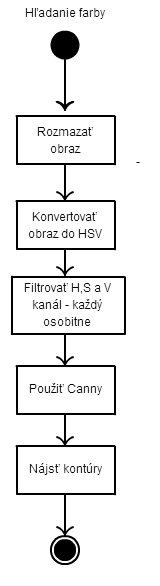
\includegraphics[width=0.3\textwidth,natwidth=160,natheight=586]{hladanie_farby.jpg}
\vspace{-20pt}
\caption{Algoritmus vyhľadávania farby v obraze}
\vspace{-10pt}
\label{hladanie_farby}
\end{figure}
\paragraph{}
Na začiatok by sa mal vstup(bitmapa) konvertovať na binárnu maticu.
\paragraph{}
Najväčšia výhoda dopravného značenia je, že je silne kontrastné od ostatného prostredia.
Túto vlastnosť môžeme perfektne využiť v náš prospech a pomocou pomocou rozmazania obrazu, môžeme dosieliť to,
že sa zbavíme slabších kontú hneď na začiatku. V OpenCV je pre rozmazávanie obrazu na výber viacero metód,
no my použijeme matódu \emph{GaussianBlur}, ktorá už názvom prezrádza použitie známeho filtra \emph{Gaussian blur}
\paragraph{}
Keďže sa snažíme dostať náš vstupný obraz do formátu HSV, o ktorú sa stará funkcionalita \emph{cvtColor} 
potrebujeme mu nastaviť vstup tak, aby obraz vedel bez problémov spracovať. 
Keďže na väčšine mobilných zariadení prichádza do zariadenia obraz vo formáte RGBA, ďalší krok bude nepríklad konvertovanie formátu RGBA na formát RGB.
\paragraph{}
Ďalej bude nasledovať samotná konverzia obrazu do HSV pomocou už spomínanej metódy \emph{cvtColor}.
\paragraph{}
Ďalší krok bude spracovať každý kanál farebného modelu HSV samostatne. Ako prvý spracujeme \emph{Hue} kanál, ktorý sa stará o farebný odtien každého pixelu.
\emph{Hue} Farba sa v tomto kanáli určuje podľa stupňov. 
Primárne sa začína na stupni 0$^\circ$, čo predstavuje zelenú farbu, postupne prechádza do modrej,
ktorá sa nachádza na 120$^\circ$ stupňoch z kade prechádza cez červenú na 240$^\circ$ a keďže je to model kruhový, vracia sa do zelenej na 360$^\circ$.
Pomocou funkcie \emph{inRange} by nemal byť problém určiť rozhranie stupňov, ktoré sme schopný akceptovať ako hľadanú farbu pre hľadané naše dopravné značenia.
Ďalší kanál je \emph{Saturation}, ktorý predstavuje sýtosť farby. Táto sýtosť sa vyjadruje v percentách, kde 0\% predstavuje šedú a 100\% je plne sýta farba.\cite{hsv_wiki_cz} 
V našom prípade je postacuje metóda \emph{threshold}. Posledný kanál \emph{Value} vyjadruje hodnotu jasu.
Keďže v praxi znamená znižovanie jasu pridávanie čiernej do základnej farby,
pre hľadanie červenej farby na dopravnom značení nie je potrebné s týmto kanálom pracovať, lebo červená farba použitá na dopravných značeniach je pomerne svetlá.
Pri hľadaní modrej je túto farbu potrebné trochu stmaviť a tak použijeme opäť funkciu \emph{threshold}.
\paragraph{}
Na koniec potrebujeme dostať len kontúry hľadanej farby. 
Najpr si budeme musieť spojiť jednotlivé kanály späť do jednej binárnej matice použitím metódy \emph{Canny}. 
Po tomto kroku by nám mali ostať len čierny obraz a biele škvrny predstavujúce červenú farbu v požadovanom rozsahu.
Z týchto bielych objektov, budeme potrebovať len okraje a tak použijeme metódu \emph{findContours}, ktorá sa postará o to, že dostaneme pole kontúr z celého obrazu.
S týmito kontúrami potom ďalej pracujeme a rozoznávame z nich hľadané útvary.
\subsubsection{Návrh algoritmu pre detekciu kruhov}
\paragraph{}
Pri detekcii dopravného značenia v tvare kruhu, je dôležité počítať s tým, že nehľadáme úplný kruh. Kruhové dopravné značenia sú vyrábané ako dokonalý kruh,
no pri ich rozpoznávaní si je potrené uvedomiť, že na objekt sa pozeráme z rôznych uhlov. Táto skutočnosť nám prináša do prolematiky dôležitý fakt,
že v skutočnosti to nie sú kruhy čo hľadáme, ale sú to elipsy. Celý algoritmus je možné vidieť na orázku č. \ref{hladanie_kruhov}

%% otekanie textu
%%\begin{wrapfigure}{r}{0.55\textwidth}
%%	\begin{center}
%%		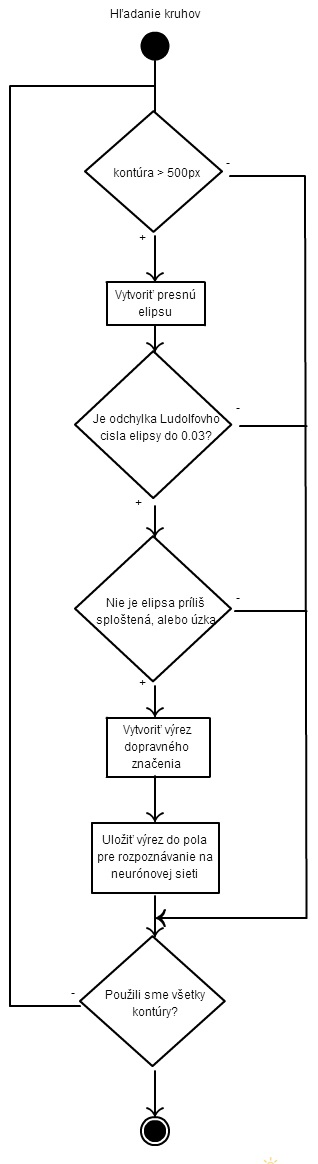
\includegraphics[width=0.4\textwidth,natwidth=318,natheight=1164]{hladanie_kruhov.jpg}
%%	\end{center}
%%	\vspace{-20pt}
%%  	\caption{Algoritmus vyhľadávania kruhov}
%%  	\vspace{-10pt}
%%  	\label{hladanie_kruhov}
%%\end{wrapfigure}
\begin{figure}[p]
\centering
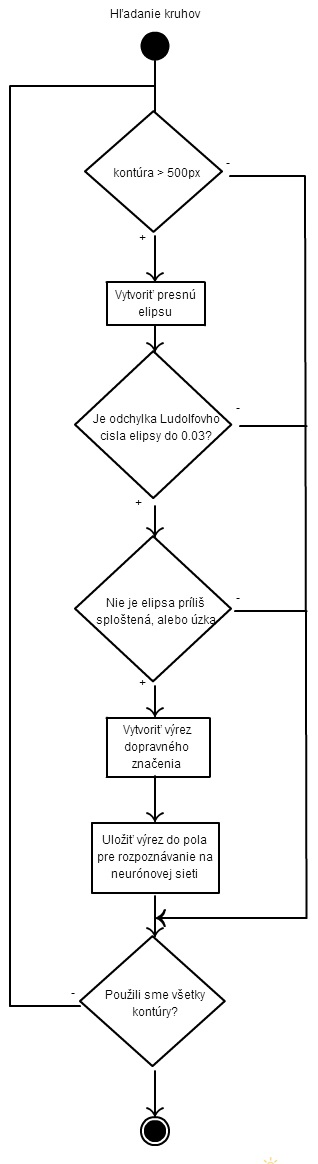
\includegraphics[width=0.38\textwidth,natwidth=318,natheight=1164]{hladanie_kruhov.jpg}
\vspace{-20pt}
\caption{Algoritmus vyhľadávania kruhov v obraze}
\vspace{-10pt}
\label{hladanie_kruhov}
\end{figure}

\paragraph{}
Keďže v predchádzajúcej kapitole sme si navrhli riešenie, ktoré nám vracia len kontúry hľadanej farby, môžeme pokračovať od tohto bodu.
Ako prvé si spravíme cyklus, ktorým budeme prechádzať všetky naše vyhľadané kontúry farieb. Aby sme eliminovali počet prebytočných kontúr, 
je potrené spracovávať čo najrelevantnejšie výsledky. Tento úkon vykoná metóda \emph{contourArea}, vďaka ktorej budeme posielať na ďalšie spracovanie len kontúry väčšie ako 500 pixelov.
\paragraph{}
Vzhľadom na to, že výsledky, ktoré dostávame ešte nemôžeme nazvať elipsami, musíme si naše kontúry na elipsy upraviť.
Tento úkon vykonáva metóda \emph{fitEllipse}, ktorá upraví kostrbaté kontúry, ktoré sa aspoň trochu podobajú elipse, na matematicky presnú elipsu.
\paragraph{}
Keď už máme detekované elipsy, nastáva posledný krok, a tým krokom je, určiť si toleranciu elipsy dopravného značenia, ktorú vyhľadávam.
Táto tolerancia, je vlastne tolerancia nepresnosti, pri výpočte Ludolfovho čísla. 
Ďalším krokom je tak výpočet už spomínaného ludolfovho čísla a následné overenie jeho nepresnosti. 
Pokiaľ je výsledná hodnota vyhovujúca, nájdený objekt vyrežeme, a zasielame na rozpoznanie neurónovej sieti, ktorá zistí o akú značku sa presne jedná.
\paragraph{}
Výpočet Ludolfovho čísla:
\begin{align*}
          \pi = \frac{o}{d} \\
\end{align*}
Úprava výpočtu Ludolfovho čísla pre elipsu:
\begin{align*}
          p = \frac{o}{d} = \frac{o}{(\frac{1}{2} y) * ( \frac{1}{2} x)} \\
\end{align*}
Získanie tolerancie:
\begin{align*}
          \pi - p < 0.03 \\
\end{align*}
%%vzorec
%%citacie z knih matematiky
\paragraph{}
Pre určovanie tolerancie elipsy, je možné použiť ešte jednu metódu, a tou je overovanie podľa osí. 
Pokiaľ je x-ová os dvoj-násobne väčšia ako y-ová, ide už o elipsu, ktorú by sme ďalej len ťažko identifikovali. 
Takýto nežiaduci stav môže nastať, pokiaľ sa na značku pozeráme na dopravné značenie z príliž veľkého uhlu.
\paragraph{}
Dva nežiaduce stavy tvaru dopravného značenia:
\begin{align*}
		  \text{ 1.) }
          \frac{\frac{1}{2} x}{\frac{1}{2} y} > 2  \\
          \text{ 2.) }
          \frac{\frac{1}{2} y}{\frac{1}{2} x} > 2  \\
\end{align*}
%%\subsubsection{Návrh algoritmu pre detekciu trojuholnikov}
%%\subsubsection{Návrh algoritmu pre detekciu štvorcov}
\subsection{Návrh objektov - UML}
\paragraph{}
Algoritmy, ktoré boli navrhnuté, je potrebne správne zakomponovať do objektovo orientovaného modelu našej android aplikácie.
Je potrebné si správne navrhnúť ako budú jednotlivé algoritmy a funkcionality rozdelené do tried a taktiež aj to, ako budú triedy medzi sebou spolupracovať.
Celá štruktúra je najlepšie viditeľná na obrázku \ref{uml_objects_diagram}.
\begin{itemize}
  \item \textbf{SurfaceView} - Táto trieda je v jadre Android OS, ale je si potrebné vysvetliť jej probližnú funkcionalitu, keďže z nej priamo dedíme a upravujeme ju v ďalších triedach našej aplikácie.
  Poskytuje špecializovanú kresliacu plochu. Podoba tejto plochy sa dá meniť, dá sa jednoducho meniť napríklad veľkosť alebo samotné umiestnenie. \cite{android_dev}
  \item \textbf{Activity} - Táto trieda je taktiež priamo v jadre Android OS, ale keďže z nej taktiež dedíme, vasvetlíme si jej hlavný princíp.
  Táto trieda má na starosti komunikáciu s užívateľom. Všetko čo užívateľ s aplikáciou spraví, napríklad čo sa stane s aplikáciou pokiaľ užívateľ pozastaví priebeh vykonávania, alebo čo sa bude diať po výbere jednotlivých položiek v menu. \cite{android_dev}
  \item \textbf{BaseClass} - Táto trieda dedí z triedy \emph{SurfaceView} a nastavuje našu plochu. Keďže na našej aplikácii máme v pláne mať na ploche hlavne pohľad z kamery, v tejto triede sa staráme o všetky správne nastavenia kamery a zoprazenia pre hlavnú plochu aplikácie.
  \item \textbf{ActivityView} - Trieda dedí z triedy \emph{Activity}. V tejto aplikácii sa nastavujú všetky akcie ktoré v našej android aplikácii môžu nastať a taktiež aj naše hlavné menu z ktorého si užívateľ vyberá akcie.
  \item \textbf{Detection} - Je to hlavná trieda zodpovedná za rozpoznanie jednotlivých objektov, nastavujeme v nej taktiež rôzne parametre, ktoré sa použijú neskôr v triedach, ktoré z našej triedy \emph{Detection} dedia.
  \item \textbf{Color} - Trieda \emph{Color} bude dediť z \emph{Detection}. Jej hlavná úloha je rozpoznávať jednotlivé farby.
  \item \textbf{Shape} - Trieda \emph{Shape} bude dediť z \emph{Detection}. Jej hlavná úloha je rozpoznávať tvary z obrazu.
  \item \textbf{Traffic} - Trieda \emph{Traffic} bude taktiež dediť z triedy \emph{Detection}. Jej hlavná úloha je rozpoznávať dopravné značenia. Využíva na to spoluprácu tried \emph{Shape} a \emph{Color}.
\end{itemize}
\begin{figure}[p]
\centering
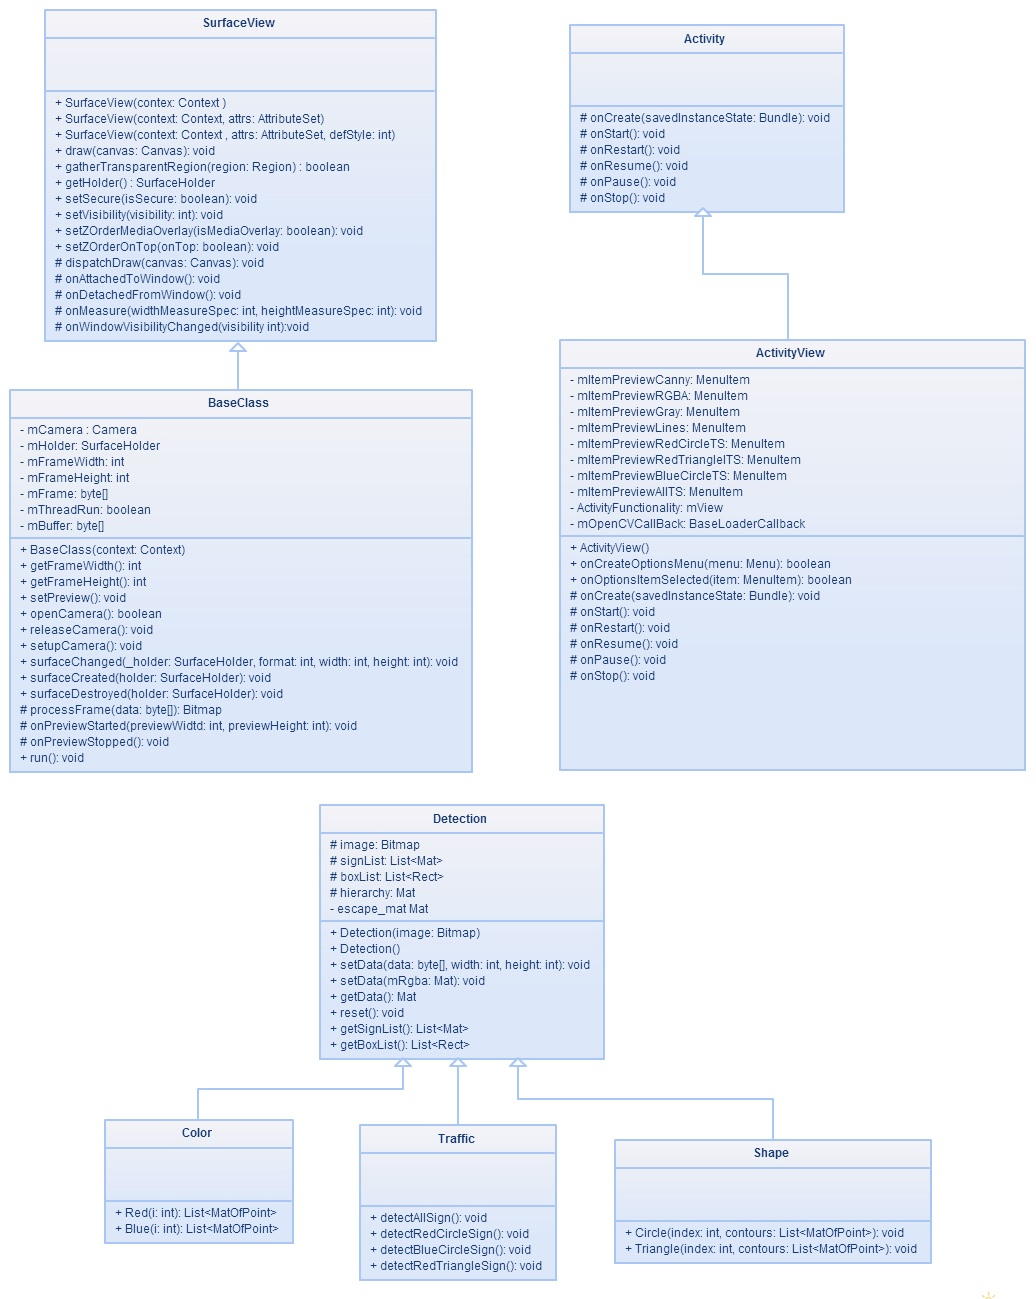
\includegraphics[width=1\textwidth,natwidth=800,natheight=1000]{uml_objects.jpg}
\vspace{-10pt}
\caption{Návrh objektov Android aplikácie}
\vspace{-10pt}
\label{uml_objects_diagram}
\end{figure}
\subsection{Návrh užívteľského prostredia}
\paragraph{}
Prostredie aplikácie bude veľmi jednoduché. Celé rozhranie, bude pozostávať z dvoch častí. Jedna časť bude naša plocha, tam sa budú graficky znázorňovať nájdené objekty, v našom prípade dorpavné značenia, ale taktiež aj rôzne filtre, ktoré budeme chcieť prezentovať ako ukážku.
Druhá časť bude menu, v ktorom si užívateľ bude vyberať z možností ktoré tam budú a následne sa budú vykonávať rôzne. V menu bude napríklad prepínanie rôznych filtrov alebo spôsobov vyhľadávania dopravných značení.
\section{Implementácia}
\paragraph{}
V tejto sekcii sa budem snažiť popísať implementáciu a správne nastavenie technológií, ktoré sa v aplikácii využijú.
\subsection{Android}
\subsection{Implementácia Opencv}
\subsection{Postup}
\subsubsection{BaseClass}
\subsubsection{ActivityView}
\subsubsection{Detection}
\subsubsection{Color}
\subsubsection{Shape}
\subsubsection{Traffic}

\section{Výsledky aplikácie}
\subsection{Detekcia kruhových značiek}
\subsubsection{Značky modrej farby}
\subsubsection{Značky červenej farby}

\section{Záver}

\bibliography{bach}
\bibliographystyle{plain}

\end{document}
